\documentclass[UTF8,adobefonts]{ctexart}

\title{矩阵在LPQ算法中的应用}
\author{王洪俊,2014010003}
\date{2014.10.1}
\def\Re{\mathop{\rm Re}}
\def\Im{\mathop{\rm Im}}
\usepackage{natbib}   %% 使用bibtex做索引文献时需要引入
\usepackage{graphicx}  %% 插入图片时需要引入
\usepackage{epstopdf}  %% 插入eps格式图片,并且使用pdflatex编译时需要引入,用latex编译时不需要引入
\usepackage{CJKutf8}   %% 使用中文目录标题需要引入
\usepackage{lineno}     %% 在伪代码中使用行号时需要引入
\usepackage{indentfirst}  %% 中文首行缩进需要引入
\usepackage[unicode]{hyperref} %%实现交叉引用,目录书签需要引入

\usepackage{amsmath}  %%使用数学公式时需要引入
\usepackage{algorithm}  %%写伪代码时需要引入
\usepackage{algorithmicx}  %%写伪代码需要引入
\usepackage[noend]{algpseudocode}  %%写伪代码需要引入
\usepackage{multirow}      %%表格中需要跨行单元格时需要引入
\usepackage{bm}
\usepackage{amsmath}
\usepackage{amssymb}
\newtheorem{theorem}{定理}[section]   %%重定义theorem命令
\newtheorem{lemma}{引理}[section]
\newtheorem{definition}{定义}[section]
\newtheorem{corollary}[theorem]{推论}
\floatname{algorithm}{算法}
\renewcommand{\algorithmicrequire}{\textbf{Input:}}
\renewcommand{\algorithmicensure}{\textbf{Output:}}

\begin{document}
\maketitle      %%生成标题
\pdfbookmark[3]{content}{section.1}   %%生成pdf的书签,3为书签层次,content为书签名,seciton.1为定位点,可以不用。

\section{概述}
现实生活中的图像中通常会表现表现出一些重复出现的样式,他们被称之为纹理特征.对这些纹理特征的分析在计算机视觉领域有着非常重要的作用,它的一些应用包括:表面鉴定,医学影象分析,遥感图像分析等等.在一些应用中,我们得到的图像不可避免地受到一些噪声影响产生失真.其中有一类失真现象为图像的模糊现象.模糊可能来自于相对运动,对焦错位或者大气湍流.由于图像去模糊非常困难,而且同时会引入其他的失真,我们在现实生活中需要一种对于模糊图像同样健壮的算法来分析图像纹理特征.

局部相位量化(Local Phase Quantization, LPQ)算法是由Ville Ojansivu提出的一种纹理分析算法,它可以对于模糊图像保持其健壮性.它是由对图像的离散傅里叶变换(DFT)的相位特征在局部域进行量化来描述图像的纹理的.LPQ算法产生的特征输出可以保证其对中心对称模糊的健壮性,这包括相对运动,对焦错位或者大气湍流产生的模糊.LPQ算子首先在局部上对每个像素进行计算,然后将全图象的结果以直方图表示.其表示方法与局部二进制特征(Local Binary Pattern,LBP)相似.而LBP算法也是纹理分析中一个常用算法.本文将介绍LPQ算法以及矩阵表示,矩阵分析在其中的作用.

\section{模糊图像的相位谱分析}\label{sec2} 
假设$f(\mathbf{x}):\mathbb{R}^2 \mapsto \mathbb{R}$代表一个在$\mathbb{R}$下的一副图像的函数值.在空间域下的一个模糊函数$f$对于图像的影响可以表示为
\begin{equation}\label{eq:1}
g(\mathbf{x})=(f*h)(\mathbf{x})
\end{equation}
其中"*"表示二维卷积,$g(\mathbf{x})$表示在$\mathbb{R}$下的一副模糊图像,$h(\mathbf{x}):\mathbb{R}^2 \mapsto \mathbb{R}$是模糊函数的点扩张函数(point spread function, PSF).

在频率域,(\ref{eq:1})式可以转化成
\begin{equation}\label{eq:2}
G(\mathbf{u})=F(\mathbf{u}) \cdot H(\mathbf{u})
\end{equation}
其中$G(\mathbf{u}),F(\mathbf{u}),H(\mathbf{u})$分别表示$g(\mathbf{x}),f(\mathbf{x}),h(\mathbf{x})$的傅里叶变换.而(\ref{eq:2})式可以进一步变换为幅度和角度的表示方式
\begin{equation}\label{eq:3}
\begin{split}
 |G(\mathbf{u})| =| F(\mathbf{u})| \cdot |H(\mathbf{u})| \\
\angle G(\mathbf{u})=\angle F(\mathbf{u}) + \angle H(\mathbf{u})
\end{split}
\end{equation}
其中$|\cdot|$代表幅值(绝对值),而$\angle$代表相位角度.

(\ref{eq:3})式表示模糊函数将同时作用于图像的幅值和相位角.但是,如果我们假定$h(\mathbf{x})$是中心对称的,即$h(\mathbf{x})=h(\mathbf{-x})$,那么其傅里叶变换$H(\mathbf{u})$将为实值,所以由傅里叶变换的奇偶虚实性质,可以得到
  \begin{equation}\label{eq:4}
      \angle H(\mathbf{u})=      
      \left\{
       \begin{array}{l}
       0, H(\mathbf{u}) \le 0   \\
       \pi, H(\mathbf{u}) < 0  \\
       \end{array}
      \right.
      \end{equation}

 \begin{equation}\label{eq:5}
      \angle G(\mathbf{u})=      
      \left\{
       \begin{array}{l}
       \angle F(\mathbf{u})\qquad,H(\mathbf{u}) \le 0   \\
       \angle F(\mathbf{u})+\pi, H(\mathbf{u}) < 0 \\
       \end{array}
      \right.
      \end{equation}




换句话说,满足$H(\mathbf{u})$为正的那些频率区域,我们得到图像$G(\mathbf{u})$的相位对于中心对称模糊是不受任何影响的.对于相对运动,对焦错位产生的模糊,我们认为模糊函数$h(\mathbf{x})$为矩形,它们在频域(sinc函数)的第一个过零点内可以保证为正.大气湍流产生的模糊我们认为其为高斯函数,它在整个频域中均为正值.图\ref{psf}展示了集中中心对称模糊PSF以及他们对应傅里叶变换的例子. \cite{brahnam2014local}
\begin{figure}[h]
\centering
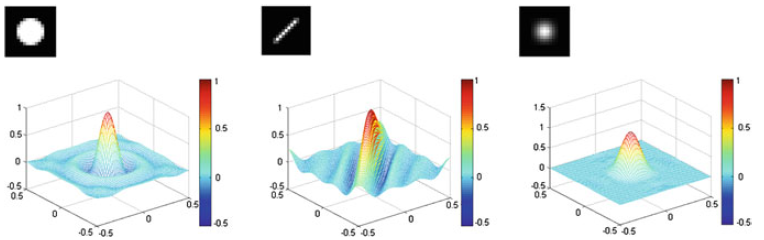
\includegraphics[height=3cm]{psf.png}

\caption{几种模糊函数PSF的例子,从左到右为:对焦错位,相对运动及高斯模糊}
\label{psf}
\end{figure}

\section{LPQ算法}
\subsection{短时傅里叶变换(STFT)}
LPQ算法是基于第\ref{sec2}章讨论的傅里叶相位谱对于中心对称模糊的健壮性的.它使用在局部图像上做二维DFT提取的信息作为第一步骤.更准确的说,是对图像的每一个像素用短时傅里叶变换(STFT)在其$M \times M$个临近像素内进行一下变换
\begin{equation}\label{eq:6}
F(\mathbf{u,x})=\sum_{\mathbf{y} \in \mathcal{N}_\mathbf{x}} f(\mathbf{x}-\mathbf{y})e^{-j2\pi \mathbf{u}^T \mathbf{y}}=\mathbf{w}^T_\mathbf{u} \mathbf{f_x}
\end{equation}

其中$\mathbf{w}_\mathbf{u}$是二维DFT变换在频率$\mathbf{u}$的基函数,而$\mathbf{f}_\mathbf{x}$是一个包含从$\mathcal{N}_\mathbf{x}$选出的所有$M^2$个图像样本.

在LPQ算法中,我们只考虑四个频率域上的基函数,它们分别是$\mathbf{u}_1 = [a,0]^T$,$\mathbf{u}_2 = [a,a]^T$,$\mathbf{u}_1 = [0,a]^T$,$\mathbf{u}_1 = [a,-a]^T$.其中$a$代表满足条件\ref{eqn:5}的第一个过零点内的某点.我们令
\begin{equation}\label{eq:7}
F_\mathbf{x}^c=[F(\mathbf{u_1,x}),F(\mathbf{u_2,x}),F(\mathbf{u_3,x}),F(\mathbf{u_4,x})]
\end{equation}
同时
\begin{equation}\label{eq:8}
F_\mathbf{x}=[\Re\{F_\mathbf{x}^c\},\Im\{F_\mathbf{x}^c\}]^T
\end{equation}
其中$\Re\{\cdot\},\Im\{\cdot\}$分别代表一个复数的实部和虚部.对应的$8 \times M^2$变换矩阵应该是
\begin{equation}\label{eq:9}
\mathbf{W}=[\Re\{\mathbf{w}_\mathbf{u_1},\mathbf{w}_\mathbf{u_2},\mathbf{w}_\mathbf{u_3},\mathbf{w}_\mathbf{u_4}\},\Im\{\mathbf{w}_\mathbf{u_1},\mathbf{w}_\mathbf{u_2},\mathbf{w}_\mathbf{u_3},\mathbf{w}_\mathbf{u_4}\}]^T
\end{equation}
所以我们得到
\begin{equation}\label{eq:10}
F_\mathbf{x}=\mathbf{Wf_x}
\end{equation}


\subsection{矩阵系数的统计分析}
我们假设图像在时域的表示$f(\mathbf{x})$是一阶马尔可夫过程,其中相邻像素的相关系数为$\rho$,并且其每个样本的方差为$\sigma^2$.所以,位置$\mathbf{x}_i$和$\mathbf{x}_j$处的相关系数为
\begin{equation}\label{eq:11}
\sigma_{ij} = \rho^{\Vert \mathbf{x}_i-\mathbf{x}_j \Vert}
\end{equation}
其中$\Vert \cdot \Vert$为$L-2$范数.同样的道理,在整个图像上的相关系数矩阵可以表示为
\begin{equation}\label{eq:12}
\mathbf{C}=\begin{bmatrix}
1 & \sigma_{12}  &  \cdots  &  \sigma_{1M}\\
\sigma_{21} & 1  &  \cdots  &  \sigma_{2M}\\
\vdots & \vdots & \ddots & \vdots\\
\sigma_{M1} &  \sigma_{M2}  &  \cdots  & 1
\end{bmatrix}
\end{equation}

所以,对于变换系数向量$F_\mathbf{x}$的相关矩阵可以通过下式得到
\begin{equation}\label{eq:13}
\mathbf{D}=\mathbf{WCW}^T
\end{equation}

我们很容易发现当$\rho>0$时,$\mathbf{D}$不是一个对角阵,所以系数应该是存在相关关系的.

\subsection{去相关与量化}
在进行量化之前,我们先把我们得到的信息去相关,因为对于统计独立的样本进行标量量化可以最大程度地保持有用信息.我们假设样本服从高斯分布,通过以下的白化变换可以使系数统计独立:
\begin{equation}\label{eq:14}
\mathbf{G_x}=\mathbf{V}^T\mathbf{F_x}
\end{equation}
其中$\mathbf{V}$是单位正交矩阵,可以通过对$\mathbf{D}$做SVD分解得到:
\begin{equation}\label{eq:15}
\mathbf{D}=\mathbf{U \Sigma V}^T
\end{equation}

需要注意对固定的$\rho$,矩阵$\mathbf{V}$可以提前求出.

现在,我们已经对图像中的所有像素都计算出$\mathbf{G_x}$了,我们接下来把得到的向量通过一个简单的标量量化过程:
\begin{equation}\label{eq:16}
      q_j=      
      \left\{
       \begin{array}{l}
       1, g_j \le 0   \\
       0, \text{其他}  \\
       \end{array}
      \right.
      \end{equation}

其中$g_j$为$\mathbf{G_x}$的第$j$个元素.量化之后的系数可以使用二进制编码用0-255中的一个整数来表示
\begin{equation}\label{eq:17}
b_j=\sum_{j=1}^8 q_j 2^{j-1}
\end{equation}

最后,对于图像每个像素都这么做,并得到的直方图,我们就可以使用这个256维的向量来作为特征向量表示整幅图的特征.

\section{总结}
在总结前,我们提一下一个细节,在公式\ref{eq:8}中,我们把图像特征分为实部和虚部,这一步相当于对图像的相位做量化,把相位表示为四个象限中的一个,而不是具体的角度,这么做实际上是由于相位量化不会对图像的纹理特征产生较大的影响,例如Cameraman图像经过量化前后对比如下图所示.\cite{brahnam2014local}
\begin{figure}[h]
\centering
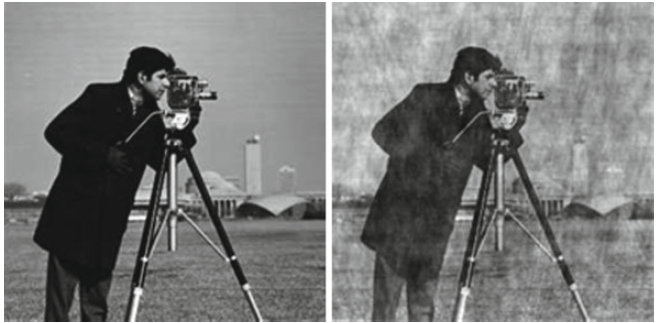
\includegraphics[height=3cm]{cameraman.png}

\caption{Cameraman图像原图(左),以及相位量化后的图(右)}
\label{cm}
\end{figure}

我们看到,在本文中矩阵的表示贯穿全文,方便了作者和读者,此外文中提到的白化算法的原理也是基于矩阵计算中相当重要的一个奇异值分解SVD算法,可见学好矩阵的重要性.
\nocite{heikkila2014local,ojansivu2008blur}
\bibliographystyle{plain}
\bibliography{reference}  %%插入索引文献
\end{document}
